% Opener for the tower cities reference plan: line up for the photo (five animals of different heights in a row)
% Build: pdflatex photo-line.tex in a scratch directory, then copy to ../reference-tower-cities-opener.pdf
% Every puzzle here is checked for exactly one answer by photo-line_check.py.
\documentclass[11pt]{article}
\usepackage[letterpaper,margin=0.5in]{geometry}
\usepackage[T1]{fontenc}
\usepackage[default]{sourcesanspro}
\usepackage{tikz}
\pagestyle{empty}
\setlength{\parindent}{0pt}
\definecolor{c1}{HTML}{F2C318}\definecolor{c2}{HTML}{3B73D6}
\definecolor{c3}{HTML}{D83A3A}\definecolor{c4}{HTML}{3BA55C}
\definecolor{c5}{HTML}{7E4BB0}
% \tower{x}{height}{colour}{name}: a tower of cubes standing on y = 0, its name below
\newcommand{\tower}[4]{%
  \foreach \k in {1,...,#2} {\fill[#3!40!white,draw=#3!70!black,line width=0.7pt] (#1,\k*0.42-0.42) rectangle ++(0.42,0.42);}
  \node[font=\small\bfseries,anchor=north] at (#1+0.21,-0.05) {#4};}
\newenvironment{half}{\begin{minipage}[t][0.475\textheight][t]{\linewidth}\large}{\end{minipage}}
\newcommand{\cutline}{\par\noindent\begin{tikzpicture}\draw[dashed,gray] (0,0)--(\linewidth-1pt,0);\end{tikzpicture}\par\vspace{0.3in}}
\newcommand{\heading}[1]{{\LARGE\bfseries #1}\hfill {\normalsize Name:} \rule{1.8in}{0.4pt}\par\medskip}
% heights picture for n animals, then the empty line of n places
\newcommand{\fiveheights}{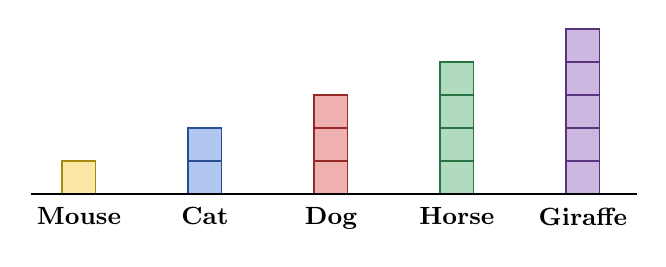
\begin{tikzpicture}
  \tower{0}{1}{c1}{Mouse}\tower{1.6}{2}{c2}{Cat}\tower{3.2}{3}{c3}{Dog}
  \tower{4.8}{4}{c4}{Horse}\tower{6.4}{5}{c5}{Giraffe}
  \draw[line width=0.6pt] (-0.4,0)--(7.3,0);\end{tikzpicture}}
\newcommand{\place}[1]{\draw[line width=1pt,rounded corners=3pt] (#1,0) rectangle ++(3.1,1.3);}
\newcommand{\fiveplaces}{\begin{center}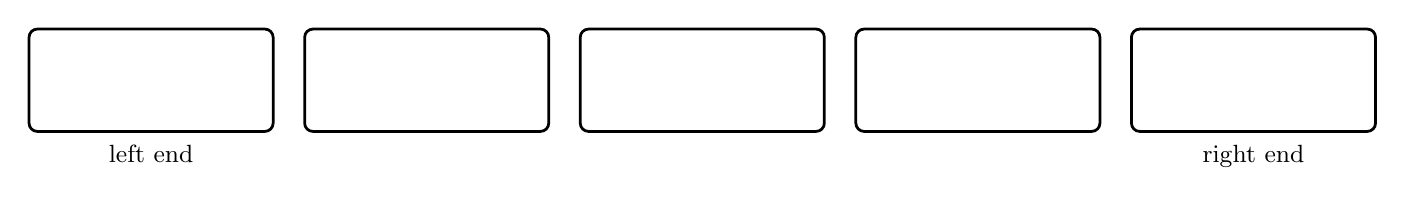
\begin{tikzpicture}
  \place{0}\place{3.5}\place{7}\place{10.5}\place{14}
  \node[font=\small,anchor=north] at (1.55,-0.05) {left end};
  \node[font=\small,anchor=north] at (15.55,-0.05) {right end};\end{tikzpicture}\end{center}}
\newcommand{\mainpuzzle}{%
  \heading{Line up for the photo}
  \begin{minipage}[b]{0.52\linewidth}
  Five animals stand in a line for a photo. The picture shows how tall each one is.
  Write each animal's name in its place in the line.
  \end{minipage}\hfill
  \begin{minipage}[b]{0.44\linewidth}\raggedleft\fiveheights\end{minipage}
  \fiveplaces
  \begin{enumerate}\setlength{\itemsep}{1pt}\setlength{\topsep}{2pt}
  \item Horse stands in the middle.
  \item Dog stands at one end of the line.
  \item Mouse stands between two taller animals.
  \item Mouse stands right next to Cat.
  \item The animal at the left end is shorter than the animal at the right end.
  \end{enumerate}
  \textbf{Done?} Cross out clue 5. How many answers are there now? Write a new clue that makes it exactly one again.}
\begin{document}
\begin{half}\mainpuzzle\end{half}
\cutline
\begin{half}\mainpuzzle\end{half}
\newpage
\begin{half}
\heading{Line up for the photo (three animals)}
\begin{minipage}[b]{0.6\linewidth}
Three animals stand in a line for a photo. The picture shows how tall each one is.
Write each animal's name in its place in the line.
\end{minipage}\hfill
\begin{minipage}[b]{0.34\linewidth}\raggedleft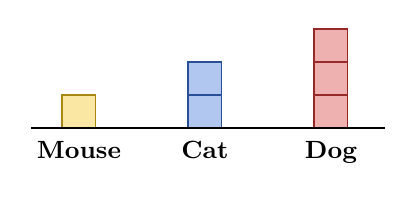
\begin{tikzpicture}
  \tower{0}{1}{c1}{Mouse}\tower{1.6}{2}{c2}{Cat}\tower{3.2}{3}{c3}{Dog}
  \draw[line width=0.6pt] (-0.4,0)--(4.1,0);\end{tikzpicture}\end{minipage}
\begin{center}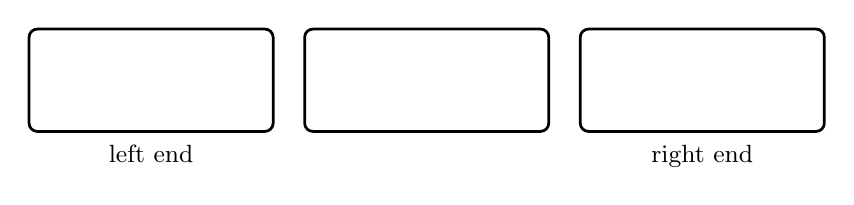
\begin{tikzpicture}
  \place{0}\place{3.5}\place{7}
  \node[font=\small,anchor=north] at (1.55,-0.05) {left end};
  \node[font=\small,anchor=north] at (8.55,-0.05) {right end};\end{tikzpicture}\end{center}
\begin{enumerate}\setlength{\itemsep}{1pt}\setlength{\topsep}{2pt}
\item The tallest animal stands at the right end.
\item Mouse stands between two taller animals.
\end{enumerate}
\textbf{Done?} Try the five-animal puzzle.
\end{half}
\cutline
\begin{half}
\heading{Line up for the photo (no place given)}
\begin{minipage}[b]{0.52\linewidth}
Five animals stand in a line for a photo. The picture shows how tall each one is.
Write each animal's name in its place in the line. No clue names a place in the line.
\end{minipage}\hfill
\begin{minipage}[b]{0.44\linewidth}\raggedleft\fiveheights\end{minipage}
\fiveplaces
\begin{enumerate}\setlength{\itemsep}{1pt}\setlength{\topsep}{2pt}
\item Every animal taller than Cat stands somewhere to the right of Cat.
\item Cat stands right next to a shorter animal.
\item Horse stands right next to Mouse.
\item The two tallest animals stand side by side.
\end{enumerate}
\textbf{Done?} Write your own five-animal puzzle with exactly one answer, and give it to a friend.
\end{half}
\end{document}
